\chapter{Methodology}
%lessons learned in iteration steps, that is new knowledge you want to share, step of insight


The Delft Systems Approach, In 't Veld


Explore environment
Define objectives

Define alternatives

Confront and tune

Develop and organize

Control and transform??


TOI single disciplinary approach, choosen, part of multi- : Tech, Org, Inf., focus on tech.


\section{Explore environment}
% learn about domain
% current state of technology
% what others before me have researched and accomplished

Various initiatives have been started to deal with one or both of these problems.
Figure \ref{fig:youbroketheinternet} shows a mapping of projects that are or have been working on that.
%From re-decentralized: top projects that match/compare.
\\
\begin{figure}[h]
	\centering
	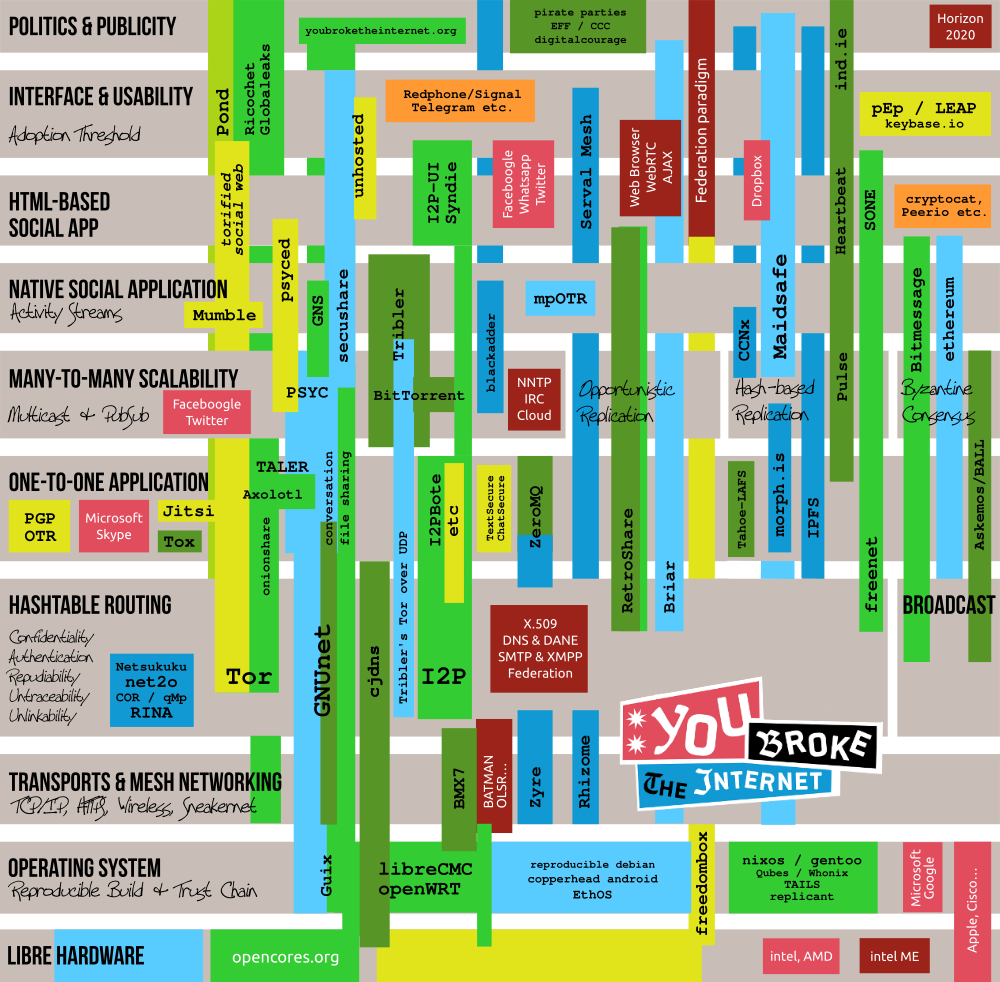
\includegraphics[width=\textwidth]{youbroketheinternet}
	\caption{Map of projects trying to fix the Internet according to youbroketheinternet.org, last updated October 2015\\
		\\
		Colour coding:\\
		\\
		\textcolor[RGB]{51,204,51}{Green:} Projects that are available today.\\
		\textcolor[RGB]{86,149,38}{Dark green:} Projects that are available, but are not fully protective of meta-data.\\
		\textcolor[RGB]{89,204,255}{Blue:} Projects in development.\\
		\textcolor[RGB]{17,153,211}{Dark blue:} Projects in development which will have little or no protection of meta-data (but that does not mean they can't be an excellent piece in the general puzzle).\\
		\textcolor[RGB]{226,228,27}{Yellow:} Projects that may be okay but depend too much on the security of servers.\\
		\textcolor[RGB]{255,153,51}{Orange:} Products whose end-to-end encrypting client side has been open-sourced but whose server side remains proprietary.\\
		\textcolor[RGB]{225,77,93}{Red:} Brands that currently occupy the respective layers with unsafe technology.\\
		\textcolor[RGB]{155,35,25}{Dark red:} Possibly cool but unsafe technologies that we need to replace.}
	\label{fig:youbroketheinternet}
\end{figure}

% Youtube screenshot, GNUnet

%%SKIP live streaming stuff below:
%being first
%engineering perfection
%time to market
%popularity
%make a difference
%Tribler mobile vs periscope
%fully functional prototype, but poor user interface (unpolished)
%real world impact proven insufficient
%we want to change the world implicit


\subsection{Tribler} %desktop version
% tribler and dispersy intro, what is it (read thesis independently)
%EXPLAIN what has been done to fix attack-reselience, VOD, self-organising, etc...

Tribler introduces a server-less video-sharing platform with privacy enhancing technologies and giving a Youtube-like, social media experience at the same time.
The capability of hiding your identity is greatly advantageous to the user if his or her human rights are violated, like free speech.

The server-less technique of Tribler is resistant to Internet kill-switches that are typically deployed for the purpose of censorship.

%what is the gap?
%GAP: no connection between puzzle pieces, that actually works on mobile



















Social media on phones

You want to express freedom of expression with that all the time % Normative, assumption of this thesis



Existing apps use central server design
Vulnarable for Internet kill switches and censorship

Offline viral spreading image (hacking lab)


How I did the work
What you have done told by what you did not do.
No answer completely, with tests that I did, but what I tested says this.... and makes it reasonable to say probably yes.


Image of what I got in the end and what I got in the beginning next to each other.


Is the main question legitimate?


What is the problem this VOD platform solves?


Regulatory perspective, out of scope
Ethical, out of scope


What do we want? VOD
What is already there? p4a
What is the gap? my work

How can we develop an autonomous and anonymous VOD platform with existing python code base that is ()user friendly /) working on a mobile platform and which is resistant to Internet kill-switches?

autonomous, not dependent on outside stuff
user friendly, power draw, special permissions

multi-coin, mobile data, nodes/hops



Imperative programming has limitations
Reactive fits mobile paradigm better


Iterations, waterfall?
Delft system approach:
Systeem -> Functional Design -> alternatives -> choose ->Prototype implementation
																									 |
|																									|
------			 validation				 <----------------------------------------

KPI 's, speed, availability, ...
or
App is done
Now: multi-criteria analysis of all other apps and mine



What is VOD?
What does working on mobile phone mean?
What are the existing modules we re-use?
What is missing? (gap)
What are the possible solutions?
Is this prototype a verified solution to main problem desc.?


this is depth first analysis now.

NOT product description



maybe problem description in an image, like system diagram


